\documentclass[twoside]{book}

% Packages required by doxygen
\usepackage{fixltx2e}
\usepackage{calc}
\usepackage{doxygen}
\usepackage[export]{adjustbox} % also loads graphicx
\usepackage{graphicx}
\usepackage[utf8]{inputenc}
\usepackage{makeidx}
\usepackage{multicol}
\usepackage{multirow}
\PassOptionsToPackage{warn}{textcomp}
\usepackage{textcomp}
\usepackage[nointegrals]{wasysym}
\usepackage[table]{xcolor}

% Font selection
\usepackage[T1]{fontenc}
\usepackage[scaled=.90]{helvet}
\usepackage{courier}
\usepackage{amssymb}
\usepackage{sectsty}
\renewcommand{\familydefault}{\sfdefault}
\allsectionsfont{%
  \fontseries{bc}\selectfont%
  \color{darkgray}%
}
\renewcommand{\DoxyLabelFont}{%
  \fontseries{bc}\selectfont%
  \color{darkgray}%
}
\newcommand{\+}{\discretionary{\mbox{\scriptsize$\hookleftarrow$}}{}{}}

% Page & text layout
\usepackage{geometry}
\geometry{%
  a4paper,%
  top=2.5cm,%
  bottom=2.5cm,%
  left=2.5cm,%
  right=2.5cm%
}
\tolerance=750
\hfuzz=15pt
\hbadness=750
\setlength{\emergencystretch}{15pt}
\setlength{\parindent}{0cm}
\setlength{\parskip}{0.2cm}
\makeatletter
\renewcommand{\paragraph}{%
  \@startsection{paragraph}{4}{0ex}{-1.0ex}{1.0ex}{%
    \normalfont\normalsize\bfseries\SS@parafont%
  }%
}
\renewcommand{\subparagraph}{%
  \@startsection{subparagraph}{5}{0ex}{-1.0ex}{1.0ex}{%
    \normalfont\normalsize\bfseries\SS@subparafont%
  }%
}
\makeatother

% Headers & footers
\usepackage{fancyhdr}
\pagestyle{fancyplain}
\fancyhead[LE]{\fancyplain{}{\bfseries\thepage}}
\fancyhead[CE]{\fancyplain{}{}}
\fancyhead[RE]{\fancyplain{}{\bfseries\leftmark}}
\fancyhead[LO]{\fancyplain{}{\bfseries\rightmark}}
\fancyhead[CO]{\fancyplain{}{}}
\fancyhead[RO]{\fancyplain{}{\bfseries\thepage}}
\fancyfoot[LE]{\fancyplain{}{}}
\fancyfoot[CE]{\fancyplain{}{}}
\fancyfoot[RE]{\fancyplain{}{\bfseries\scriptsize Generated on Mon Nov 23 2015 16\+:13\+:39 for My Project by Doxygen }}
\fancyfoot[LO]{\fancyplain{}{\bfseries\scriptsize Generated on Mon Nov 23 2015 16\+:13\+:39 for My Project by Doxygen }}
\fancyfoot[CO]{\fancyplain{}{}}
\fancyfoot[RO]{\fancyplain{}{}}
\renewcommand{\footrulewidth}{0.4pt}
\renewcommand{\chaptermark}[1]{%
  \markboth{#1}{}%
}
\renewcommand{\sectionmark}[1]{%
  \markright{\thesection\ #1}%
}

% Indices & bibliography
\usepackage{natbib}
\usepackage[titles]{tocloft}
\setcounter{tocdepth}{3}
\setcounter{secnumdepth}{5}
\makeindex

% Hyperlinks (required, but should be loaded last)
\usepackage{ifpdf}
\ifpdf
  \usepackage[pdftex,pagebackref=true]{hyperref}
\else
  \usepackage[ps2pdf,pagebackref=true]{hyperref}
\fi
\hypersetup{%
  colorlinks=true,%
  linkcolor=blue,%
  citecolor=blue,%
  unicode%
}

% Custom commands
\newcommand{\clearemptydoublepage}{%
  \newpage{\pagestyle{empty}\cleardoublepage}%
}


%===== C O N T E N T S =====

\begin{document}

% Titlepage & ToC
\hypersetup{pageanchor=false,
             bookmarks=true,
             bookmarksnumbered=true,
             pdfencoding=unicode
            }
\pagenumbering{roman}
\begin{titlepage}
\vspace*{7cm}
\begin{center}%
{\Large My Project }\\
\vspace*{1cm}
{\large Generated by Doxygen 1.8.10}\\
\vspace*{0.5cm}
{\small Mon Nov 23 2015 16:13:39}\\
\end{center}
\end{titlepage}
\clearemptydoublepage
\tableofcontents
\clearemptydoublepage
\pagenumbering{arabic}
\hypersetup{pageanchor=true}

%--- Begin generated contents ---
\chapter{Hierarchical Index}
\section{Class Hierarchy}
This inheritance list is sorted roughly, but not completely, alphabetically\+:\begin{DoxyCompactList}
\item \contentsline{section}{cl\+\_\+figures}{\pageref{classcl__figures}}{}
\begin{DoxyCompactList}
\item \contentsline{section}{cl\+\_\+ball}{\pageref{classcl__ball}}{}
\item \contentsline{section}{cl\+\_\+square}{\pageref{classcl__square}}{}
\end{DoxyCompactList}
\item \contentsline{section}{cl\+\_\+operations}{\pageref{classcl__operations}}{}
\begin{DoxyCompactList}
\item \contentsline{section}{cl\+\_\+intersection}{\pageref{classcl__intersection}}{}
\end{DoxyCompactList}
\end{DoxyCompactList}

\chapter{Class Index}
\section{Class List}
Here are the classes, structs, unions and interfaces with brief descriptions\+:\begin{DoxyCompactList}
\item\contentsline{section}{\hyperlink{classcl__ball}{cl\+\_\+ball} }{\pageref{classcl__ball}}{}
\item\contentsline{section}{\hyperlink{classcl__figures}{cl\+\_\+figures} }{\pageref{classcl__figures}}{}
\item\contentsline{section}{\hyperlink{classcl__intersection}{cl\+\_\+intersection} }{\pageref{classcl__intersection}}{}
\item\contentsline{section}{\hyperlink{classcl__operations}{cl\+\_\+operations} }{\pageref{classcl__operations}}{}
\item\contentsline{section}{\hyperlink{classcl__square}{cl\+\_\+square} }{\pageref{classcl__square}}{}
\end{DoxyCompactList}

\chapter{Class Documentation}
\hypertarget{classcl__ball}{}\section{cl\+\_\+ball Class Reference}
\label{classcl__ball}\index{cl\+\_\+ball@{cl\+\_\+ball}}
Inheritance diagram for cl\+\_\+ball\+:\begin{figure}[H]
\begin{center}
\leavevmode
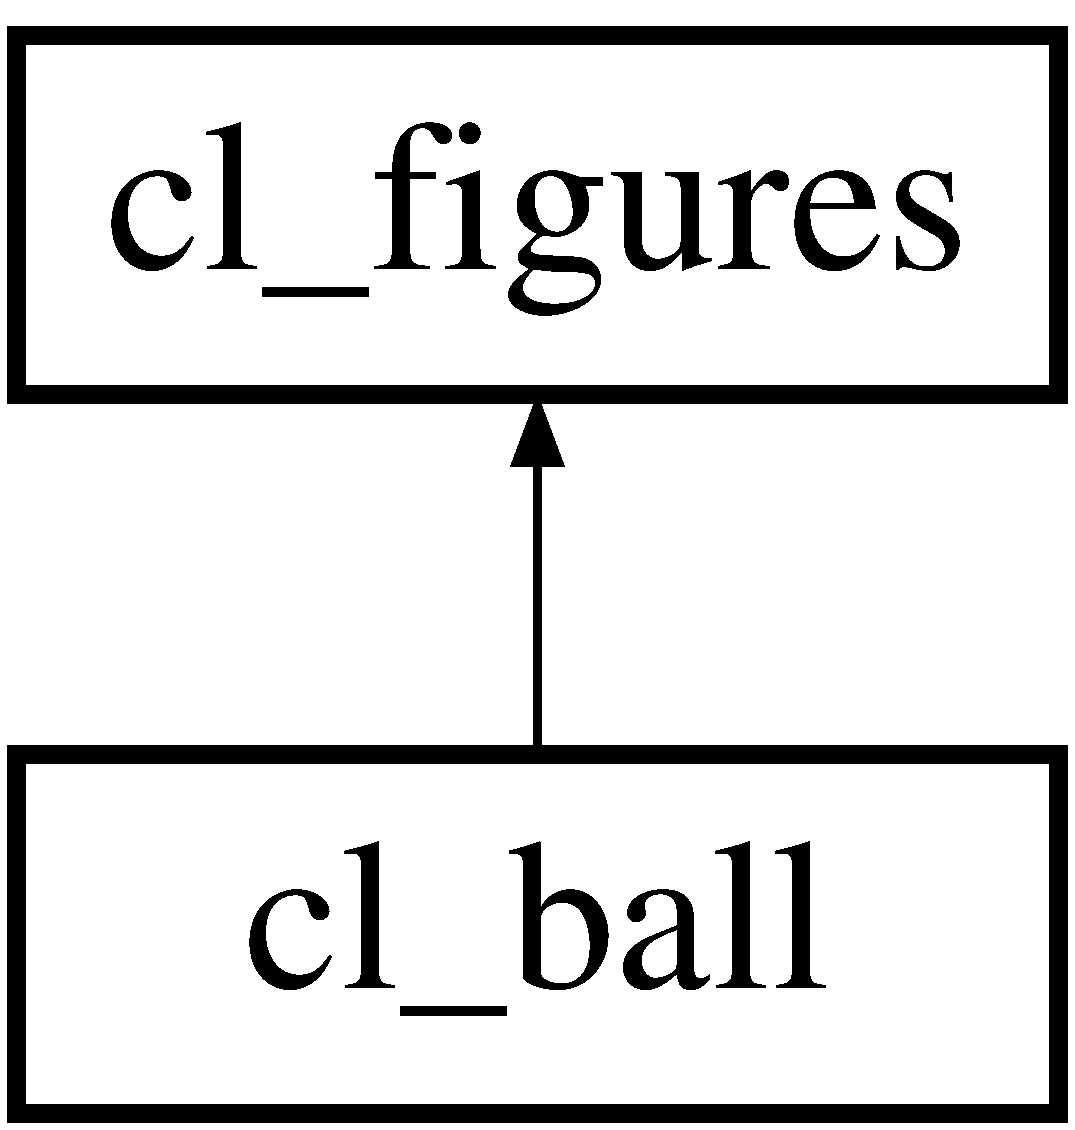
\includegraphics[height=2.000000cm]{classcl__ball}
\end{center}
\end{figure}
\subsection*{Public Member Functions}
{\bf }\par
\begin{DoxyCompactItemize}
\item 
\hyperlink{classcl__ball_a097ce75b4ce4af7534abe10aa71bf918}{cl\+\_\+ball} ()
\begin{DoxyCompactList}\small\item\em Default Construtor. \end{DoxyCompactList}\item 
\hyperlink{classcl__ball_aa98bdf4ffd4ac3cb35b84686234c6a2e}{cl\+\_\+ball} (float x, float y, float z, float r)
\begin{DoxyCompactList}\small\item\em Parameter Constructor (Kreis) \end{DoxyCompactList}\end{DoxyCompactItemize}

{\bf }\par
\begin{DoxyCompactItemize}
\item 
void \hyperlink{classcl__ball_a6d13f50c176344c4b199b11a52737866}{set\+Radius} (float R)
\begin{DoxyCompactList}\small\item\em (void) set\+Radius \end{DoxyCompactList}\item 
float \hyperlink{classcl__ball_a6c2ec7629e03361ec6e4676e560cf5a8}{get\+Radius} ()
\begin{DoxyCompactList}\small\item\em (float) get\+Radius \end{DoxyCompactList}\end{DoxyCompactItemize}

{\bf }\par
\begin{DoxyCompactItemize}
\item 
bool \hyperlink{classcl__ball_a6936133de95a8022e064e1abca6e2916}{is\+In\+Ball} (std\+::vector$<$ float $>$ a)
\begin{DoxyCompactList}\small\item\em (bool) is\+In \end{DoxyCompactList}\end{DoxyCompactItemize}

{\bf }\par
\begin{DoxyCompactItemize}
\item 
void \hyperlink{classcl__figures_af1c498c43e5f302f9701f99d4407e6f0}{set\+Pos\+X} (float pos\+X)
\begin{DoxyCompactList}\small\item\em (void) set\+Pos\+X, set\+Pos\+Y, set\+Pos\+Z \end{DoxyCompactList}\item 
void \hyperlink{classcl__figures_ae07156aefb81f1a9b460e743f8f8c410}{set\+Pos\+Y} (float pos\+Y)
\item 
\hypertarget{classcl__figures_aaf722642edb1bd71e56e5005ad509182}{}void {\bfseries set\+Pos\+Z} (float pos\+Z)\label{classcl__figures_aaf722642edb1bd71e56e5005ad509182}

\end{DoxyCompactItemize}

{\bf }\par
\begin{DoxyCompactItemize}
\item 
void \hyperlink{classcl__figures_a00276ccac945306e2c65c0dcc7a7f558}{move\+To} (float pos\+X, float pos\+Y, float pos\+Z)
\begin{DoxyCompactList}\small\item\em (void) move\+To \end{DoxyCompactList}\end{DoxyCompactItemize}

{\bf }\par
\begin{DoxyCompactItemize}
\item 
float \hyperlink{classcl__figures_a4aff7e34bc5d177eb6332d1a40ea69ca}{get\+Pos\+X} ()
\begin{DoxyCompactList}\small\item\em (float) get\+X, get\+Y, get\+Z \end{DoxyCompactList}\item 
\hypertarget{classcl__figures_a8f5e37378abacd6075ab9df52abc109d}{}float {\bfseries get\+Pos\+Y} ()\label{classcl__figures_a8f5e37378abacd6075ab9df52abc109d}

\item 
\hypertarget{classcl__figures_a5e4861620e8f28d19d5ac29e71792b46}{}float {\bfseries get\+Pos\+Z} ()\label{classcl__figures_a5e4861620e8f28d19d5ac29e71792b46}

\end{DoxyCompactItemize}

\subsection*{Public Attributes}
\begin{DoxyCompactItemize}
\item 
float \hyperlink{classcl__ball_a313bac2803bc95538febbd3f81a3b353}{m\+\_\+radius}
\end{DoxyCompactItemize}
\subsection*{Protected Attributes}
\begin{DoxyCompactItemize}
\item 
std\+::vector$<$ float $>$ \hyperlink{classcl__figures_a8db478de16f1fa9005f66c821f1c9231}{m\+\_\+center\+Point}
\item 
std\+::vector$<$ float $>$ \hyperlink{classcl__figures_a2213b88adc79462eb87457ffb18b17a2}{m\+\_\+pos}
\end{DoxyCompactItemize}


\subsection{Constructor \& Destructor Documentation}
\hypertarget{classcl__ball_a097ce75b4ce4af7534abe10aa71bf918}{}\index{cl\+\_\+ball@{cl\+\_\+ball}!cl\+\_\+ball@{cl\+\_\+ball}}
\index{cl\+\_\+ball@{cl\+\_\+ball}!cl\+\_\+ball@{cl\+\_\+ball}}
\subsubsection[{cl\+\_\+ball()}]{\setlength{\rightskip}{0pt plus 5cm}cl\+\_\+ball\+::cl\+\_\+ball (
\begin{DoxyParamCaption}
{}
\end{DoxyParamCaption}
)}\label{classcl__ball_a097ce75b4ce4af7534abe10aa71bf918}


Default Construtor. 

Default Konstruktor der Klasse \hyperlink{classcl__ball}{cl\+\_\+ball}.

initialisiert einen Kreis mit den Parametern \#m\+\_\+pos\+X und \#m\+\_\+pos\+Y \hypertarget{classcl__ball_aa98bdf4ffd4ac3cb35b84686234c6a2e}{}\index{cl\+\_\+ball@{cl\+\_\+ball}!cl\+\_\+ball@{cl\+\_\+ball}}
\index{cl\+\_\+ball@{cl\+\_\+ball}!cl\+\_\+ball@{cl\+\_\+ball}}
\subsubsection[{cl\+\_\+ball(float x, float y, float z, float r)}]{\setlength{\rightskip}{0pt plus 5cm}cl\+\_\+ball\+::cl\+\_\+ball (
\begin{DoxyParamCaption}
\item[{float}]{x, }
\item[{float}]{y, }
\item[{float}]{z, }
\item[{float}]{r}
\end{DoxyParamCaption}
)}\label{classcl__ball_aa98bdf4ffd4ac3cb35b84686234c6a2e}


Parameter Constructor (Kreis) 

Kreis wird initialisiert durch Mittelpunkt und Raduis 
\begin{DoxyParams}[1]{Parameters}
\mbox{\tt in}  & {\em pos\+X} & (float) Position auf x-\/\+Achse \\
\hline
\mbox{\tt in}  & {\em pos\+Y} & (float) Position auf y-\/\+Achse \\
\hline
\mbox{\tt in}  & {\em pos\+Z} & /float) Position auf z-\/\+Achse\\
\hline
\end{DoxyParams}
Kreis wird initialisiert durch Mittelpunkt und Radius 
\begin{DoxyParams}[1]{Parameters}
\mbox{\tt in}  & {\em pos\+X} & (float) Position auf x-\/\+Achse \\
\hline
\mbox{\tt in}  & {\em pos\+Y} & (float) Position auf y-\/\+Achse \\
\hline
\mbox{\tt in}  & {\em pos\+Z} & /float) Position auf z-\/\+Achse \\
\hline
\mbox{\tt in}  & {\em r} & Radius \\
\hline
\end{DoxyParams}


\subsection{Member Function Documentation}
\hypertarget{classcl__figures_a4aff7e34bc5d177eb6332d1a40ea69ca}{}\index{cl\+\_\+ball@{cl\+\_\+ball}!get\+Pos\+X@{get\+Pos\+X}}
\index{get\+Pos\+X@{get\+Pos\+X}!cl\+\_\+ball@{cl\+\_\+ball}}
\subsubsection[{get\+Pos\+X()}]{\setlength{\rightskip}{0pt plus 5cm}float cl\+\_\+figures\+::get\+Pos\+X (
\begin{DoxyParamCaption}
{}
\end{DoxyParamCaption}
)\hspace{0.3cm}{\ttfamily [inherited]}}\label{classcl__figures_a4aff7e34bc5d177eb6332d1a40ea69ca}


(float) get\+X, get\+Y, get\+Z 

Ermittelt die Werte für die Position (x,y,z) 
\begin{DoxyParams}[1]{Parameters}
\mbox{\tt out}  & {\em m\+\_\+pos} & Position \\
\hline
\end{DoxyParams}
\begin{DoxyReturn}{Returns}
m\+\_\+pos\mbox{[}0\mbox{]} 

m\+\_\+pos\mbox{[}1\mbox{]} 

m\+\_\+pos\mbox{[}2\mbox{]} 
\end{DoxyReturn}
\hypertarget{classcl__ball_a6c2ec7629e03361ec6e4676e560cf5a8}{}\index{cl\+\_\+ball@{cl\+\_\+ball}!get\+Radius@{get\+Radius}}
\index{get\+Radius@{get\+Radius}!cl\+\_\+ball@{cl\+\_\+ball}}
\subsubsection[{get\+Radius()}]{\setlength{\rightskip}{0pt plus 5cm}float cl\+\_\+ball\+::get\+Radius (
\begin{DoxyParamCaption}
{}
\end{DoxyParamCaption}
)}\label{classcl__ball_a6c2ec7629e03361ec6e4676e560cf5a8}


(float) get\+Radius 


\begin{DoxyParams}[1]{Parameters}
\mbox{\tt out}  & {\em m\+\_\+radius} & Radius \\
\hline
\end{DoxyParams}
\begin{DoxyReturn}{Returns}
m\+\_\+radius 
\end{DoxyReturn}
\hypertarget{classcl__ball_a6936133de95a8022e064e1abca6e2916}{}\index{cl\+\_\+ball@{cl\+\_\+ball}!is\+In\+Ball@{is\+In\+Ball}}
\index{is\+In\+Ball@{is\+In\+Ball}!cl\+\_\+ball@{cl\+\_\+ball}}
\subsubsection[{is\+In\+Ball(std\+::vector$<$ float $>$ a)}]{\setlength{\rightskip}{0pt plus 5cm}bool cl\+\_\+ball\+::is\+In\+Ball (
\begin{DoxyParamCaption}
\item[{std\+::vector$<$ float $>$}]{a}
\end{DoxyParamCaption}
)}\label{classcl__ball_a6936133de95a8022e064e1abca6e2916}


(bool) is\+In 

überprüft ob sich ein Punkt a in dem Kreis befindet \begin{DoxyReturn}{Returns}
true oder false 
\end{DoxyReturn}
Der Abstand zwischen dem Mittelpunkt $(x_1,y_1)$ und dem Punkt a $(a_1,a_2)$ ist $\sqrt{(x_2-x_1)^2+(a_2-a_1)^2}$. Ist dieser Abstand kleiner als der Radius, liegt der Punkt a innerhalb des Kreises \hypertarget{classcl__figures_a00276ccac945306e2c65c0dcc7a7f558}{}\index{cl\+\_\+ball@{cl\+\_\+ball}!move\+To@{move\+To}}
\index{move\+To@{move\+To}!cl\+\_\+ball@{cl\+\_\+ball}}
\subsubsection[{move\+To(float pos\+X, float pos\+Y, float pos\+Z)}]{\setlength{\rightskip}{0pt plus 5cm}void cl\+\_\+figures\+::move\+To (
\begin{DoxyParamCaption}
\item[{float}]{pos\+X, }
\item[{float}]{pos\+Y, }
\item[{float}]{pos\+Z}
\end{DoxyParamCaption}
)\hspace{0.3cm}{\ttfamily [inherited]}}\label{classcl__figures_a00276ccac945306e2c65c0dcc7a7f558}


(void) move\+To 

Veraendert die Position des Objekts \begin{DoxySeeAlso}{See also}
\hyperlink{classcl__figures_af1c498c43e5f302f9701f99d4407e6f0}{set\+Pos\+X()} 

\hyperlink{classcl__figures_ae07156aefb81f1a9b460e743f8f8c410}{set\+Pos\+Y()} 

set\+Pos\+Z() 
\end{DoxySeeAlso}

\begin{DoxyParams}[1]{Parameters}
\mbox{\tt in}  & {\em pos\+X} & (float) zugewiesener Wert \\
\hline
\mbox{\tt in}  & {\em pos\+Y} & (float) zugewiesener Wert \\
\hline
\mbox{\tt in}  & {\em pos\+Z} & (float) zugewiesener Wert \\
\hline
\end{DoxyParams}
\hypertarget{classcl__figures_af1c498c43e5f302f9701f99d4407e6f0}{}\index{cl\+\_\+ball@{cl\+\_\+ball}!set\+Pos\+X@{set\+Pos\+X}}
\index{set\+Pos\+X@{set\+Pos\+X}!cl\+\_\+ball@{cl\+\_\+ball}}
\subsubsection[{set\+Pos\+X(float pos\+X)}]{\setlength{\rightskip}{0pt plus 5cm}void cl\+\_\+figures\+::set\+Pos\+X (
\begin{DoxyParamCaption}
\item[{float}]{pos\+X}
\end{DoxyParamCaption}
)\hspace{0.3cm}{\ttfamily [inherited]}}\label{classcl__figures_af1c498c43e5f302f9701f99d4407e6f0}


(void) set\+Pos\+X, set\+Pos\+Y, set\+Pos\+Z 

Zuweisung der Position der x-\/, y-\/ bzw. z-\/\+Achse 
\begin{DoxyParams}[1]{Parameters}
 & {\em m\+\_\+pos} & (vector$<$float$>$) Position \\
\hline
\mbox{\tt in}  & {\em pos\+X} & (float) zugewiesener Wert \\
\hline
\mbox{\tt in}  & {\em pos\+Y} & (float) zugewiesener Wert \\
\hline
\mbox{\tt in}  & {\em pos\+Z} & (float) zugewiesener Wert\\
\hline
\end{DoxyParams}
Zuweisung der Position der x bzw. y-\/\+Achse 
\begin{DoxyParams}[1]{Parameters}
\mbox{\tt in}  & {\em m\+\_\+pos} & (vector$<$float$>$) Position \\
\hline
\mbox{\tt in}  & {\em pos\+X} & (float) zugewiesener Wert \\
\hline
\mbox{\tt in}  & {\em pos\+Y} & (float) zugewiesener Wert \\
\hline
\end{DoxyParams}
\hypertarget{classcl__figures_ae07156aefb81f1a9b460e743f8f8c410}{}\index{cl\+\_\+ball@{cl\+\_\+ball}!set\+Pos\+Y@{set\+Pos\+Y}}
\index{set\+Pos\+Y@{set\+Pos\+Y}!cl\+\_\+ball@{cl\+\_\+ball}}
\subsubsection[{set\+Pos\+Y(float pos\+Y)}]{\setlength{\rightskip}{0pt plus 5cm}void cl\+\_\+figures\+::set\+Pos\+Y (
\begin{DoxyParamCaption}
\item[{float}]{pos\+Y}
\end{DoxyParamCaption}
)\hspace{0.3cm}{\ttfamily [inherited]}}\label{classcl__figures_ae07156aefb81f1a9b460e743f8f8c410}
Rahmenbedingungen? \hypertarget{classcl__ball_a6d13f50c176344c4b199b11a52737866}{}\index{cl\+\_\+ball@{cl\+\_\+ball}!set\+Radius@{set\+Radius}}
\index{set\+Radius@{set\+Radius}!cl\+\_\+ball@{cl\+\_\+ball}}
\subsubsection[{set\+Radius(float R)}]{\setlength{\rightskip}{0pt plus 5cm}void cl\+\_\+ball\+::set\+Radius (
\begin{DoxyParamCaption}
\item[{float}]{R}
\end{DoxyParamCaption}
)}\label{classcl__ball_a6d13f50c176344c4b199b11a52737866}


(void) set\+Radius 

Zuweisung des Wertes R für den Radius 
\begin{DoxyParams}[1]{Parameters}
\mbox{\tt in}  & {\em R} & (float) Radius \\
\hline
\end{DoxyParams}


\subsection{Member Data Documentation}
\hypertarget{classcl__figures_a8db478de16f1fa9005f66c821f1c9231}{}\index{cl\+\_\+ball@{cl\+\_\+ball}!m\+\_\+center\+Point@{m\+\_\+center\+Point}}
\index{m\+\_\+center\+Point@{m\+\_\+center\+Point}!cl\+\_\+ball@{cl\+\_\+ball}}
\subsubsection[{m\+\_\+center\+Point}]{\setlength{\rightskip}{0pt plus 5cm}std\+::vector$<$float$>$ cl\+\_\+figures\+::m\+\_\+center\+Point\hspace{0.3cm}{\ttfamily [protected]}, {\ttfamily [inherited]}}\label{classcl__figures_a8db478de16f1fa9005f66c821f1c9231}

\begin{DoxyParams}[1]{Parameters}
\mbox{\tt in}  & {\em m\+\_\+center\+Point} & \\
\hline
\end{DoxyParams}
\hypertarget{classcl__figures_a2213b88adc79462eb87457ffb18b17a2}{}\index{cl\+\_\+ball@{cl\+\_\+ball}!m\+\_\+pos@{m\+\_\+pos}}
\index{m\+\_\+pos@{m\+\_\+pos}!cl\+\_\+ball@{cl\+\_\+ball}}
\subsubsection[{m\+\_\+pos}]{\setlength{\rightskip}{0pt plus 5cm}std\+::vector$<$float$>$ cl\+\_\+figures\+::m\+\_\+pos\hspace{0.3cm}{\ttfamily [protected]}, {\ttfamily [inherited]}}\label{classcl__figures_a2213b88adc79462eb87457ffb18b17a2}

\begin{DoxyParams}[1]{Parameters}
\mbox{\tt in}  & {\em m\+\_\+pos} & (vector$<$float$>$) Position des Kreises \\
\hline
\end{DoxyParams}
\hypertarget{classcl__ball_a313bac2803bc95538febbd3f81a3b353}{}\index{cl\+\_\+ball@{cl\+\_\+ball}!m\+\_\+radius@{m\+\_\+radius}}
\index{m\+\_\+radius@{m\+\_\+radius}!cl\+\_\+ball@{cl\+\_\+ball}}
\subsubsection[{m\+\_\+radius}]{\setlength{\rightskip}{0pt plus 5cm}float cl\+\_\+ball\+::m\+\_\+radius}\label{classcl__ball_a313bac2803bc95538febbd3f81a3b353}

\begin{DoxyParams}[1]{Parameters}
\mbox{\tt in}  & {\em m\+\_\+radius} & (float) Radius des Kreises bzw. der Kugel \\
\hline
\end{DoxyParams}


The documentation for this class was generated from the following files\+:\begin{DoxyCompactItemize}
\item 
cl\+\_\+ball.\+h\item 
cl\+\_\+ball.\+cpp\end{DoxyCompactItemize}

\hypertarget{classcl__figures}{}\section{cl\+\_\+figures Class Reference}
\label{classcl__figures}\index{cl\+\_\+figures@{cl\+\_\+figures}}
Inheritance diagram for cl\+\_\+figures\+:\begin{figure}[H]
\begin{center}
\leavevmode
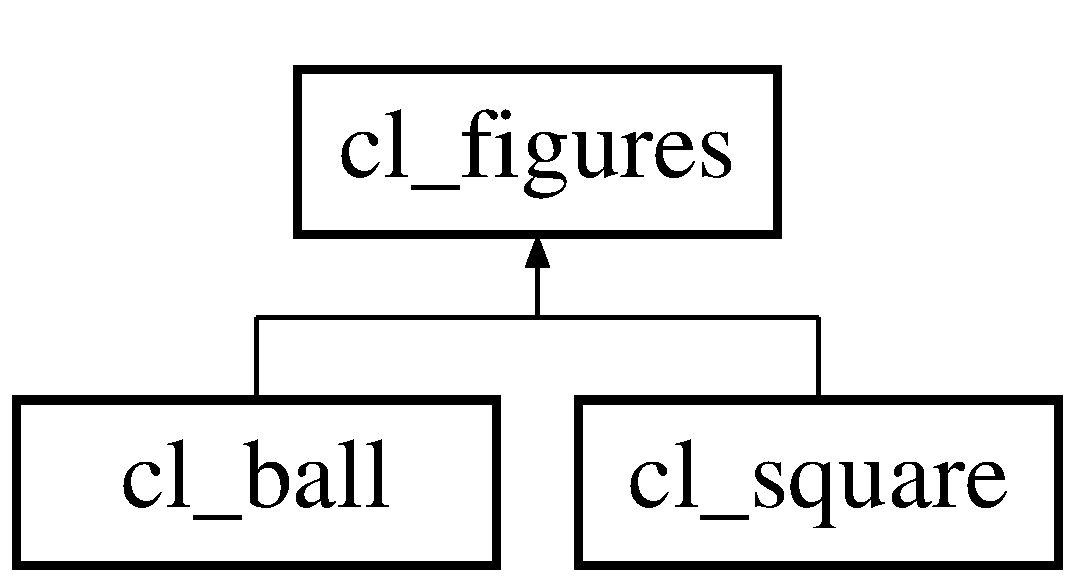
\includegraphics[height=2.000000cm]{classcl__figures}
\end{center}
\end{figure}
\subsection*{Public Member Functions}
{\bf }\par
\begin{DoxyCompactItemize}
\item 
\hyperlink{classcl__figures_ae32a5f74827021284748bb1f93ed88c0}{cl\+\_\+figures} ()
\begin{DoxyCompactList}\small\item\em Default Constructor. \end{DoxyCompactList}\item 
\hyperlink{classcl__figures_a7d40c61a6f518c59a7e4aebdbaac9ea2}{cl\+\_\+figures} (float pos\+X, float pos\+Y, float pos\+Z)
\begin{DoxyCompactList}\small\item\em Parameter Construktor (Geometrisches Objekt) \end{DoxyCompactList}\end{DoxyCompactItemize}

{\bf }\par
\begin{DoxyCompactItemize}
\item 
void \hyperlink{classcl__figures_af1c498c43e5f302f9701f99d4407e6f0}{set\+Pos\+X} (float pos\+X)
\begin{DoxyCompactList}\small\item\em (void) set\+Pos\+X, set\+Pos\+Y, set\+Pos\+Z \end{DoxyCompactList}\item 
void \hyperlink{classcl__figures_ae07156aefb81f1a9b460e743f8f8c410}{set\+Pos\+Y} (float pos\+Y)
\item 
\hypertarget{classcl__figures_aaf722642edb1bd71e56e5005ad509182}{}void {\bfseries set\+Pos\+Z} (float pos\+Z)\label{classcl__figures_aaf722642edb1bd71e56e5005ad509182}

\end{DoxyCompactItemize}

{\bf }\par
\begin{DoxyCompactItemize}
\item 
void \hyperlink{classcl__figures_a00276ccac945306e2c65c0dcc7a7f558}{move\+To} (float pos\+X, float pos\+Y, float pos\+Z)
\begin{DoxyCompactList}\small\item\em (void) move\+To \end{DoxyCompactList}\end{DoxyCompactItemize}

{\bf }\par
\begin{DoxyCompactItemize}
\item 
float \hyperlink{classcl__figures_a4aff7e34bc5d177eb6332d1a40ea69ca}{get\+Pos\+X} ()
\begin{DoxyCompactList}\small\item\em (float) get\+X, get\+Y, get\+Z \end{DoxyCompactList}\item 
\hypertarget{classcl__figures_a8f5e37378abacd6075ab9df52abc109d}{}float {\bfseries get\+Pos\+Y} ()\label{classcl__figures_a8f5e37378abacd6075ab9df52abc109d}

\item 
\hypertarget{classcl__figures_a5e4861620e8f28d19d5ac29e71792b46}{}float {\bfseries get\+Pos\+Z} ()\label{classcl__figures_a5e4861620e8f28d19d5ac29e71792b46}

\end{DoxyCompactItemize}

\subsection*{Protected Attributes}
\begin{DoxyCompactItemize}
\item 
std\+::vector$<$ float $>$ \hyperlink{classcl__figures_a8db478de16f1fa9005f66c821f1c9231}{m\+\_\+center\+Point}
\item 
std\+::vector$<$ float $>$ \hyperlink{classcl__figures_a2213b88adc79462eb87457ffb18b17a2}{m\+\_\+pos}
\end{DoxyCompactItemize}


\subsection{Constructor \& Destructor Documentation}
\hypertarget{classcl__figures_ae32a5f74827021284748bb1f93ed88c0}{}\index{cl\+\_\+figures@{cl\+\_\+figures}!cl\+\_\+figures@{cl\+\_\+figures}}
\index{cl\+\_\+figures@{cl\+\_\+figures}!cl\+\_\+figures@{cl\+\_\+figures}}
\subsubsection[{cl\+\_\+figures()}]{\setlength{\rightskip}{0pt plus 5cm}cl\+\_\+figures\+::cl\+\_\+figures (
\begin{DoxyParamCaption}
{}
\end{DoxyParamCaption}
)}\label{classcl__figures_ae32a5f74827021284748bb1f93ed88c0}


Default Constructor. 

Default Construktor. \hypertarget{classcl__figures_a7d40c61a6f518c59a7e4aebdbaac9ea2}{}\index{cl\+\_\+figures@{cl\+\_\+figures}!cl\+\_\+figures@{cl\+\_\+figures}}
\index{cl\+\_\+figures@{cl\+\_\+figures}!cl\+\_\+figures@{cl\+\_\+figures}}
\subsubsection[{cl\+\_\+figures(float pos\+X, float pos\+Y, float pos\+Z)}]{\setlength{\rightskip}{0pt plus 5cm}cl\+\_\+figures\+::cl\+\_\+figures (
\begin{DoxyParamCaption}
\item[{float}]{pos\+X, }
\item[{float}]{pos\+Y, }
\item[{float}]{pos\+Z}
\end{DoxyParamCaption}
)}\label{classcl__figures_a7d40c61a6f518c59a7e4aebdbaac9ea2}


Parameter Construktor (Geometrisches Objekt) 

Ein geometrisches Objekt wird initialisiert durch Angabe einer neuen Position 
\begin{DoxyParams}[1]{Parameters}
\mbox{\tt in}  & {\em pos\+X} & (float) Position auf x-\/\+Achse \\
\hline
\mbox{\tt in}  & {\em pos\+Y} & (float) Position auf y-\/\+Achse \\
\hline
\mbox{\tt in}  & {\em pos\+Z} & /float) Position auf z-\/\+Achse\\
\hline
\end{DoxyParams}
Ein geometrisches Objekt wird initialisiert durch Angabe einer Position 
\begin{DoxyParams}[1]{Parameters}
\mbox{\tt in}  & {\em pos\+X} & (float) Position auf x-\/\+Achse \\
\hline
\mbox{\tt in}  & {\em pos\+Y} & (float) Position auf y-\/\+Achse \\
\hline
\mbox{\tt in}  & {\em pos\+Z} & /float) Position auf z-\/\+Achse \\
\hline
\end{DoxyParams}


\subsection{Member Function Documentation}
\hypertarget{classcl__figures_a4aff7e34bc5d177eb6332d1a40ea69ca}{}\index{cl\+\_\+figures@{cl\+\_\+figures}!get\+Pos\+X@{get\+Pos\+X}}
\index{get\+Pos\+X@{get\+Pos\+X}!cl\+\_\+figures@{cl\+\_\+figures}}
\subsubsection[{get\+Pos\+X()}]{\setlength{\rightskip}{0pt plus 5cm}float cl\+\_\+figures\+::get\+Pos\+X (
\begin{DoxyParamCaption}
{}
\end{DoxyParamCaption}
)}\label{classcl__figures_a4aff7e34bc5d177eb6332d1a40ea69ca}


(float) get\+X, get\+Y, get\+Z 

Ermittelt die Werte für die Position (x,y,z) 
\begin{DoxyParams}[1]{Parameters}
\mbox{\tt out}  & {\em m\+\_\+pos} & Position \\
\hline
\end{DoxyParams}
\begin{DoxyReturn}{Returns}
m\+\_\+pos\mbox{[}0\mbox{]} 

m\+\_\+pos\mbox{[}1\mbox{]} 

m\+\_\+pos\mbox{[}2\mbox{]} 
\end{DoxyReturn}
\hypertarget{classcl__figures_a00276ccac945306e2c65c0dcc7a7f558}{}\index{cl\+\_\+figures@{cl\+\_\+figures}!move\+To@{move\+To}}
\index{move\+To@{move\+To}!cl\+\_\+figures@{cl\+\_\+figures}}
\subsubsection[{move\+To(float pos\+X, float pos\+Y, float pos\+Z)}]{\setlength{\rightskip}{0pt plus 5cm}void cl\+\_\+figures\+::move\+To (
\begin{DoxyParamCaption}
\item[{float}]{pos\+X, }
\item[{float}]{pos\+Y, }
\item[{float}]{pos\+Z}
\end{DoxyParamCaption}
)}\label{classcl__figures_a00276ccac945306e2c65c0dcc7a7f558}


(void) move\+To 

Veraendert die Position des Objekts \begin{DoxySeeAlso}{See also}
\hyperlink{classcl__figures_af1c498c43e5f302f9701f99d4407e6f0}{set\+Pos\+X()} 

\hyperlink{classcl__figures_ae07156aefb81f1a9b460e743f8f8c410}{set\+Pos\+Y()} 

set\+Pos\+Z() 
\end{DoxySeeAlso}

\begin{DoxyParams}[1]{Parameters}
\mbox{\tt in}  & {\em pos\+X} & (float) zugewiesener Wert \\
\hline
\mbox{\tt in}  & {\em pos\+Y} & (float) zugewiesener Wert \\
\hline
\mbox{\tt in}  & {\em pos\+Z} & (float) zugewiesener Wert \\
\hline
\end{DoxyParams}
\hypertarget{classcl__figures_af1c498c43e5f302f9701f99d4407e6f0}{}\index{cl\+\_\+figures@{cl\+\_\+figures}!set\+Pos\+X@{set\+Pos\+X}}
\index{set\+Pos\+X@{set\+Pos\+X}!cl\+\_\+figures@{cl\+\_\+figures}}
\subsubsection[{set\+Pos\+X(float pos\+X)}]{\setlength{\rightskip}{0pt plus 5cm}void cl\+\_\+figures\+::set\+Pos\+X (
\begin{DoxyParamCaption}
\item[{float}]{pos\+X}
\end{DoxyParamCaption}
)}\label{classcl__figures_af1c498c43e5f302f9701f99d4407e6f0}


(void) set\+Pos\+X, set\+Pos\+Y, set\+Pos\+Z 

Zuweisung der Position der x-\/, y-\/ bzw. z-\/\+Achse 
\begin{DoxyParams}[1]{Parameters}
 & {\em m\+\_\+pos} & (vector$<$float$>$) Position \\
\hline
\mbox{\tt in}  & {\em pos\+X} & (float) zugewiesener Wert \\
\hline
\mbox{\tt in}  & {\em pos\+Y} & (float) zugewiesener Wert \\
\hline
\mbox{\tt in}  & {\em pos\+Z} & (float) zugewiesener Wert\\
\hline
\end{DoxyParams}
Zuweisung der Position der x bzw. y-\/\+Achse 
\begin{DoxyParams}[1]{Parameters}
\mbox{\tt in}  & {\em m\+\_\+pos} & (vector$<$float$>$) Position \\
\hline
\mbox{\tt in}  & {\em pos\+X} & (float) zugewiesener Wert \\
\hline
\mbox{\tt in}  & {\em pos\+Y} & (float) zugewiesener Wert \\
\hline
\end{DoxyParams}
\hypertarget{classcl__figures_ae07156aefb81f1a9b460e743f8f8c410}{}\index{cl\+\_\+figures@{cl\+\_\+figures}!set\+Pos\+Y@{set\+Pos\+Y}}
\index{set\+Pos\+Y@{set\+Pos\+Y}!cl\+\_\+figures@{cl\+\_\+figures}}
\subsubsection[{set\+Pos\+Y(float pos\+Y)}]{\setlength{\rightskip}{0pt plus 5cm}void cl\+\_\+figures\+::set\+Pos\+Y (
\begin{DoxyParamCaption}
\item[{float}]{pos\+Y}
\end{DoxyParamCaption}
)}\label{classcl__figures_ae07156aefb81f1a9b460e743f8f8c410}
Rahmenbedingungen? 

\subsection{Member Data Documentation}
\hypertarget{classcl__figures_a8db478de16f1fa9005f66c821f1c9231}{}\index{cl\+\_\+figures@{cl\+\_\+figures}!m\+\_\+center\+Point@{m\+\_\+center\+Point}}
\index{m\+\_\+center\+Point@{m\+\_\+center\+Point}!cl\+\_\+figures@{cl\+\_\+figures}}
\subsubsection[{m\+\_\+center\+Point}]{\setlength{\rightskip}{0pt plus 5cm}std\+::vector$<$float$>$ cl\+\_\+figures\+::m\+\_\+center\+Point\hspace{0.3cm}{\ttfamily [protected]}}\label{classcl__figures_a8db478de16f1fa9005f66c821f1c9231}

\begin{DoxyParams}[1]{Parameters}
\mbox{\tt in}  & {\em m\+\_\+center\+Point} & \\
\hline
\end{DoxyParams}
\hypertarget{classcl__figures_a2213b88adc79462eb87457ffb18b17a2}{}\index{cl\+\_\+figures@{cl\+\_\+figures}!m\+\_\+pos@{m\+\_\+pos}}
\index{m\+\_\+pos@{m\+\_\+pos}!cl\+\_\+figures@{cl\+\_\+figures}}
\subsubsection[{m\+\_\+pos}]{\setlength{\rightskip}{0pt plus 5cm}std\+::vector$<$float$>$ cl\+\_\+figures\+::m\+\_\+pos\hspace{0.3cm}{\ttfamily [protected]}}\label{classcl__figures_a2213b88adc79462eb87457ffb18b17a2}

\begin{DoxyParams}[1]{Parameters}
\mbox{\tt in}  & {\em m\+\_\+pos} & (vector$<$float$>$) Position des Kreises \\
\hline
\end{DoxyParams}


The documentation for this class was generated from the following files\+:\begin{DoxyCompactItemize}
\item 
cl\+\_\+figures.\+h\item 
cl\+\_\+figures.\+cpp\end{DoxyCompactItemize}

\hypertarget{classcl__intersection}{}\section{cl\+\_\+intersection Class Reference}
\label{classcl__intersection}\index{cl\+\_\+intersection@{cl\+\_\+intersection}}
Inheritance diagram for cl\+\_\+intersection\+:\begin{figure}[H]
\begin{center}
\leavevmode
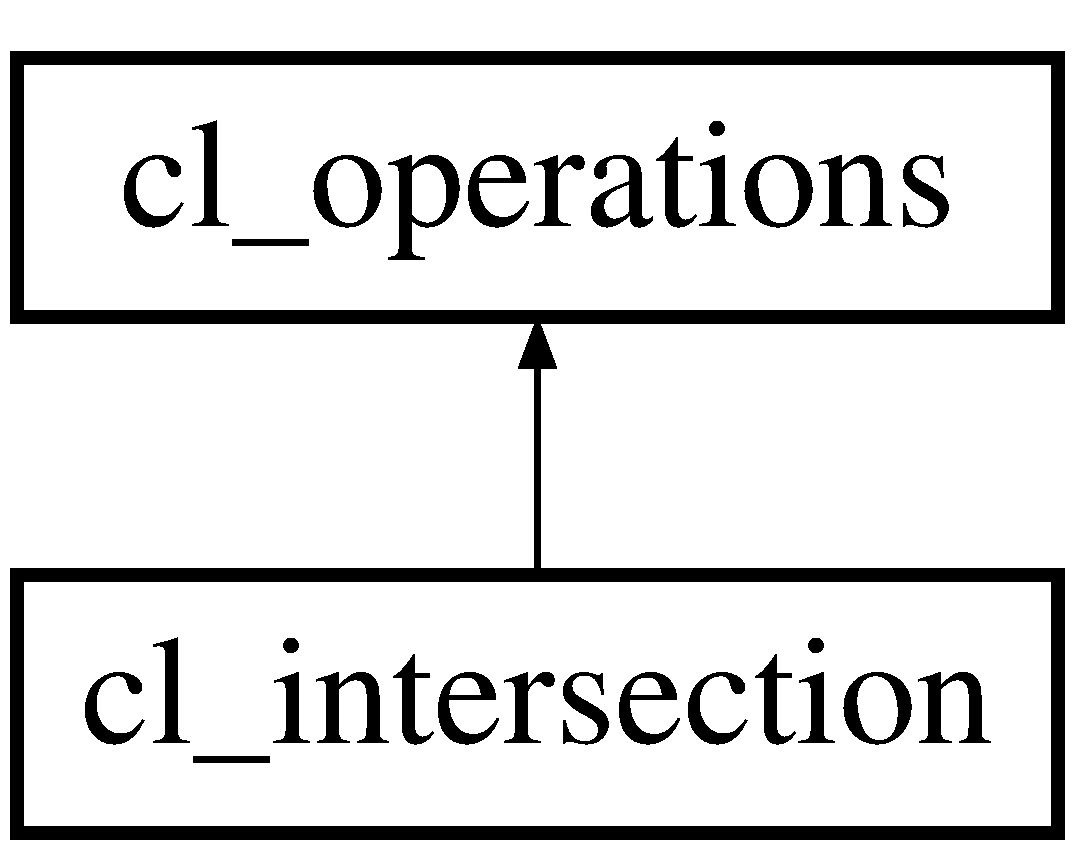
\includegraphics[height=2.000000cm]{classcl__intersection}
\end{center}
\end{figure}


The documentation for this class was generated from the following files\+:\begin{DoxyCompactItemize}
\item 
cl\+\_\+intersection.\+h\item 
cl\+\_\+intersection.\+cpp\end{DoxyCompactItemize}

\hypertarget{classcl__operations}{}\section{cl\+\_\+operations Class Reference}
\label{classcl__operations}\index{cl\+\_\+operations@{cl\+\_\+operations}}
Inheritance diagram for cl\+\_\+operations\+:\begin{figure}[H]
\begin{center}
\leavevmode
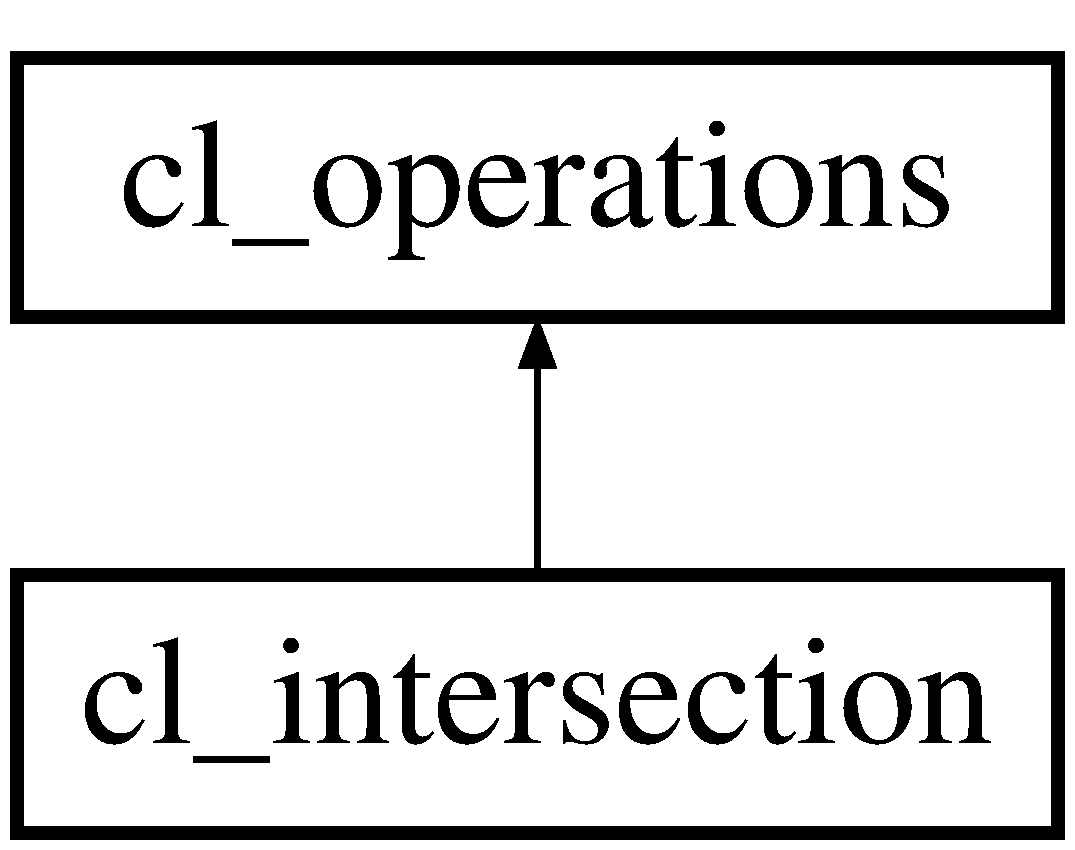
\includegraphics[height=2.000000cm]{classcl__operations}
\end{center}
\end{figure}
\subsection*{Public Member Functions}
\begin{DoxyCompactItemize}
\item 
\hypertarget{classcl__operations_a8aa98833a975207320d3f1270258f4dd}{}\hyperlink{classcl__operations_a8aa98833a975207320d3f1270258f4dd}{cl\+\_\+operations} ()\label{classcl__operations_a8aa98833a975207320d3f1270258f4dd}

\begin{DoxyCompactList}\small\item\em Default Construktor. \end{DoxyCompactList}\end{DoxyCompactItemize}


The documentation for this class was generated from the following files\+:\begin{DoxyCompactItemize}
\item 
cl\+\_\+operations.\+h\item 
cl\+\_\+operations.\+cpp\end{DoxyCompactItemize}

\hypertarget{classcl__square}{}\section{cl\+\_\+square Class Reference}
\label{classcl__square}\index{cl\+\_\+square@{cl\+\_\+square}}
Inheritance diagram for cl\+\_\+square\+:\begin{figure}[H]
\begin{center}
\leavevmode
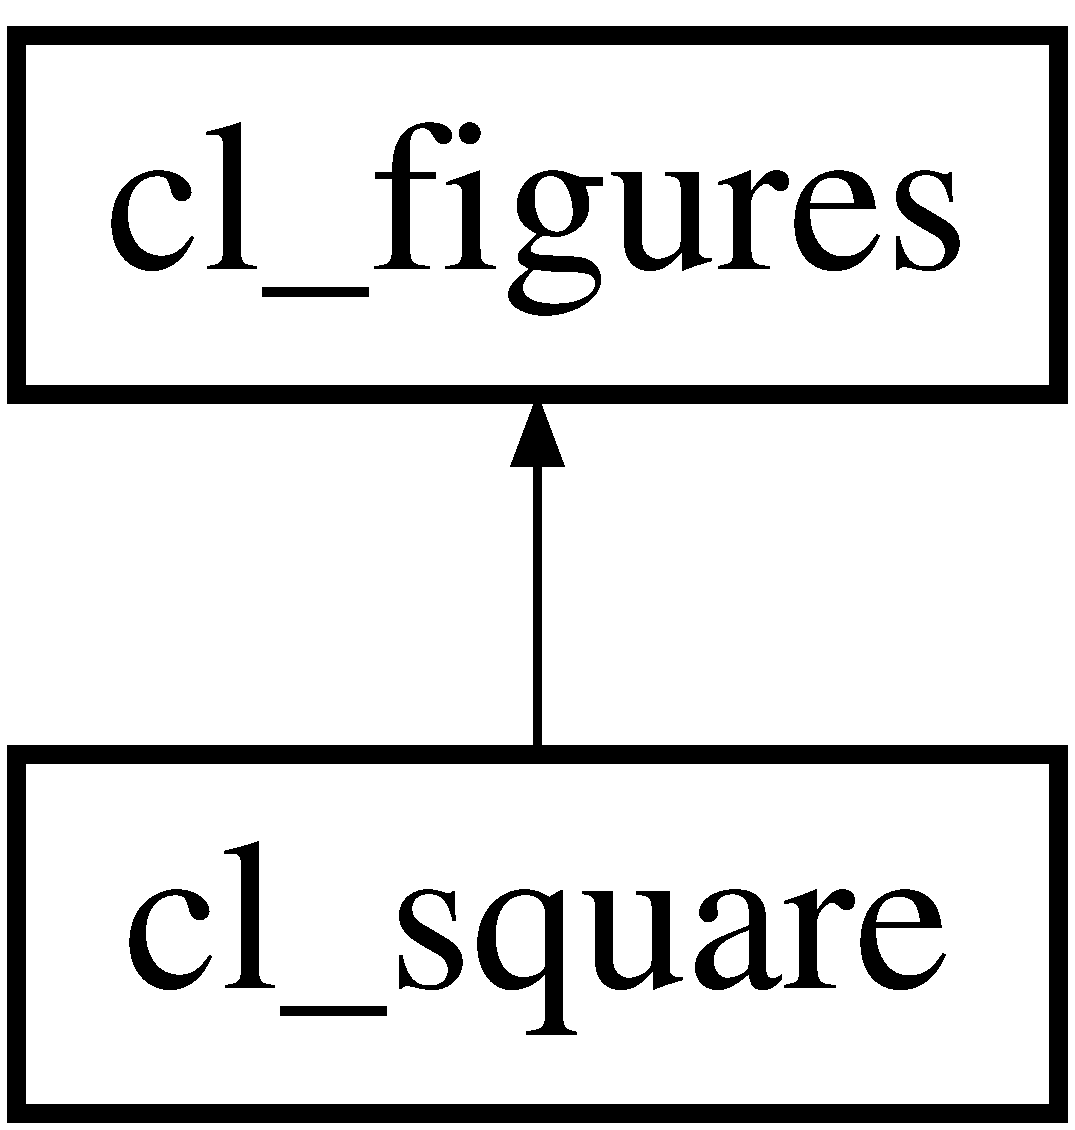
\includegraphics[height=2.000000cm]{classcl__square}
\end{center}
\end{figure}
\subsection*{Public Member Functions}
{\bf }\par
\begin{DoxyCompactItemize}
\item 
void \hyperlink{classcl__figures_af1c498c43e5f302f9701f99d4407e6f0}{set\+Pos\+X} (float pos\+X)
\begin{DoxyCompactList}\small\item\em (void) set\+Pos\+X, set\+Pos\+Y, set\+Pos\+Z \end{DoxyCompactList}\item 
void \hyperlink{classcl__figures_ae07156aefb81f1a9b460e743f8f8c410}{set\+Pos\+Y} (float pos\+Y)
\item 
\hypertarget{classcl__figures_aaf722642edb1bd71e56e5005ad509182}{}void {\bfseries set\+Pos\+Z} (float pos\+Z)\label{classcl__figures_aaf722642edb1bd71e56e5005ad509182}

\end{DoxyCompactItemize}

{\bf }\par
\begin{DoxyCompactItemize}
\item 
void \hyperlink{classcl__figures_a00276ccac945306e2c65c0dcc7a7f558}{move\+To} (float pos\+X, float pos\+Y, float pos\+Z)
\begin{DoxyCompactList}\small\item\em (void) move\+To \end{DoxyCompactList}\end{DoxyCompactItemize}

{\bf }\par
\begin{DoxyCompactItemize}
\item 
float \hyperlink{classcl__figures_a4aff7e34bc5d177eb6332d1a40ea69ca}{get\+Pos\+X} ()
\begin{DoxyCompactList}\small\item\em (float) get\+X, get\+Y, get\+Z \end{DoxyCompactList}\item 
\hypertarget{classcl__figures_a8f5e37378abacd6075ab9df52abc109d}{}float {\bfseries get\+Pos\+Y} ()\label{classcl__figures_a8f5e37378abacd6075ab9df52abc109d}

\item 
\hypertarget{classcl__figures_a5e4861620e8f28d19d5ac29e71792b46}{}float {\bfseries get\+Pos\+Z} ()\label{classcl__figures_a5e4861620e8f28d19d5ac29e71792b46}

\end{DoxyCompactItemize}

\subsection*{Protected Attributes}
\begin{DoxyCompactItemize}
\item 
std\+::vector$<$ float $>$ \hyperlink{classcl__figures_a8db478de16f1fa9005f66c821f1c9231}{m\+\_\+center\+Point}
\item 
std\+::vector$<$ float $>$ \hyperlink{classcl__figures_a2213b88adc79462eb87457ffb18b17a2}{m\+\_\+pos}
\end{DoxyCompactItemize}


\subsection{Member Function Documentation}
\hypertarget{classcl__figures_a4aff7e34bc5d177eb6332d1a40ea69ca}{}\index{cl\+\_\+square@{cl\+\_\+square}!get\+Pos\+X@{get\+Pos\+X}}
\index{get\+Pos\+X@{get\+Pos\+X}!cl\+\_\+square@{cl\+\_\+square}}
\subsubsection[{get\+Pos\+X()}]{\setlength{\rightskip}{0pt plus 5cm}float cl\+\_\+figures\+::get\+Pos\+X (
\begin{DoxyParamCaption}
{}
\end{DoxyParamCaption}
)\hspace{0.3cm}{\ttfamily [inherited]}}\label{classcl__figures_a4aff7e34bc5d177eb6332d1a40ea69ca}


(float) get\+X, get\+Y, get\+Z 

Ermittelt die Werte für die Position (x,y,z) 
\begin{DoxyParams}[1]{Parameters}
\mbox{\tt out}  & {\em m\+\_\+pos} & Position \\
\hline
\end{DoxyParams}
\begin{DoxyReturn}{Returns}
m\+\_\+pos\mbox{[}0\mbox{]} 

m\+\_\+pos\mbox{[}1\mbox{]} 

m\+\_\+pos\mbox{[}2\mbox{]} 
\end{DoxyReturn}
\hypertarget{classcl__figures_a00276ccac945306e2c65c0dcc7a7f558}{}\index{cl\+\_\+square@{cl\+\_\+square}!move\+To@{move\+To}}
\index{move\+To@{move\+To}!cl\+\_\+square@{cl\+\_\+square}}
\subsubsection[{move\+To(float pos\+X, float pos\+Y, float pos\+Z)}]{\setlength{\rightskip}{0pt plus 5cm}void cl\+\_\+figures\+::move\+To (
\begin{DoxyParamCaption}
\item[{float}]{pos\+X, }
\item[{float}]{pos\+Y, }
\item[{float}]{pos\+Z}
\end{DoxyParamCaption}
)\hspace{0.3cm}{\ttfamily [inherited]}}\label{classcl__figures_a00276ccac945306e2c65c0dcc7a7f558}


(void) move\+To 

Veraendert die Position des Objekts \begin{DoxySeeAlso}{See also}
\hyperlink{classcl__figures_af1c498c43e5f302f9701f99d4407e6f0}{set\+Pos\+X()} 

\hyperlink{classcl__figures_ae07156aefb81f1a9b460e743f8f8c410}{set\+Pos\+Y()} 

set\+Pos\+Z() 
\end{DoxySeeAlso}

\begin{DoxyParams}[1]{Parameters}
\mbox{\tt in}  & {\em pos\+X} & (float) zugewiesener Wert \\
\hline
\mbox{\tt in}  & {\em pos\+Y} & (float) zugewiesener Wert \\
\hline
\mbox{\tt in}  & {\em pos\+Z} & (float) zugewiesener Wert \\
\hline
\end{DoxyParams}
\hypertarget{classcl__figures_af1c498c43e5f302f9701f99d4407e6f0}{}\index{cl\+\_\+square@{cl\+\_\+square}!set\+Pos\+X@{set\+Pos\+X}}
\index{set\+Pos\+X@{set\+Pos\+X}!cl\+\_\+square@{cl\+\_\+square}}
\subsubsection[{set\+Pos\+X(float pos\+X)}]{\setlength{\rightskip}{0pt plus 5cm}void cl\+\_\+figures\+::set\+Pos\+X (
\begin{DoxyParamCaption}
\item[{float}]{pos\+X}
\end{DoxyParamCaption}
)\hspace{0.3cm}{\ttfamily [inherited]}}\label{classcl__figures_af1c498c43e5f302f9701f99d4407e6f0}


(void) set\+Pos\+X, set\+Pos\+Y, set\+Pos\+Z 

Zuweisung der Position der x-\/, y-\/ bzw. z-\/\+Achse 
\begin{DoxyParams}[1]{Parameters}
 & {\em m\+\_\+pos} & (vector$<$float$>$) Position \\
\hline
\mbox{\tt in}  & {\em pos\+X} & (float) zugewiesener Wert \\
\hline
\mbox{\tt in}  & {\em pos\+Y} & (float) zugewiesener Wert \\
\hline
\mbox{\tt in}  & {\em pos\+Z} & (float) zugewiesener Wert\\
\hline
\end{DoxyParams}
Zuweisung der Position der x bzw. y-\/\+Achse 
\begin{DoxyParams}[1]{Parameters}
\mbox{\tt in}  & {\em m\+\_\+pos} & (vector$<$float$>$) Position \\
\hline
\mbox{\tt in}  & {\em pos\+X} & (float) zugewiesener Wert \\
\hline
\mbox{\tt in}  & {\em pos\+Y} & (float) zugewiesener Wert \\
\hline
\end{DoxyParams}
\hypertarget{classcl__figures_ae07156aefb81f1a9b460e743f8f8c410}{}\index{cl\+\_\+square@{cl\+\_\+square}!set\+Pos\+Y@{set\+Pos\+Y}}
\index{set\+Pos\+Y@{set\+Pos\+Y}!cl\+\_\+square@{cl\+\_\+square}}
\subsubsection[{set\+Pos\+Y(float pos\+Y)}]{\setlength{\rightskip}{0pt plus 5cm}void cl\+\_\+figures\+::set\+Pos\+Y (
\begin{DoxyParamCaption}
\item[{float}]{pos\+Y}
\end{DoxyParamCaption}
)\hspace{0.3cm}{\ttfamily [inherited]}}\label{classcl__figures_ae07156aefb81f1a9b460e743f8f8c410}
Rahmenbedingungen? 

\subsection{Member Data Documentation}
\hypertarget{classcl__figures_a8db478de16f1fa9005f66c821f1c9231}{}\index{cl\+\_\+square@{cl\+\_\+square}!m\+\_\+center\+Point@{m\+\_\+center\+Point}}
\index{m\+\_\+center\+Point@{m\+\_\+center\+Point}!cl\+\_\+square@{cl\+\_\+square}}
\subsubsection[{m\+\_\+center\+Point}]{\setlength{\rightskip}{0pt plus 5cm}std\+::vector$<$float$>$ cl\+\_\+figures\+::m\+\_\+center\+Point\hspace{0.3cm}{\ttfamily [protected]}, {\ttfamily [inherited]}}\label{classcl__figures_a8db478de16f1fa9005f66c821f1c9231}

\begin{DoxyParams}[1]{Parameters}
\mbox{\tt in}  & {\em m\+\_\+center\+Point} & \\
\hline
\end{DoxyParams}
\hypertarget{classcl__figures_a2213b88adc79462eb87457ffb18b17a2}{}\index{cl\+\_\+square@{cl\+\_\+square}!m\+\_\+pos@{m\+\_\+pos}}
\index{m\+\_\+pos@{m\+\_\+pos}!cl\+\_\+square@{cl\+\_\+square}}
\subsubsection[{m\+\_\+pos}]{\setlength{\rightskip}{0pt plus 5cm}std\+::vector$<$float$>$ cl\+\_\+figures\+::m\+\_\+pos\hspace{0.3cm}{\ttfamily [protected]}, {\ttfamily [inherited]}}\label{classcl__figures_a2213b88adc79462eb87457ffb18b17a2}

\begin{DoxyParams}[1]{Parameters}
\mbox{\tt in}  & {\em m\+\_\+pos} & (vector$<$float$>$) Position des Kreises \\
\hline
\end{DoxyParams}


The documentation for this class was generated from the following files\+:\begin{DoxyCompactItemize}
\item 
cl\+\_\+square.\+h\item 
cl\+\_\+square.\+cpp\end{DoxyCompactItemize}

%--- End generated contents ---

% Index
\backmatter
\newpage
\phantomsection
\clearemptydoublepage
\addcontentsline{toc}{chapter}{Index}
\printindex

\end{document}
